\lhead{\emph{Results}} 
\chapter{Results}

The experiment was performed 16 times with 6 different people. The
results were analyzed, taking into account the previous descripted metrics
and different perspectives that are reflected in the following 5
plots that are commented on individually.

\begin{figure}[!ht]
\centering
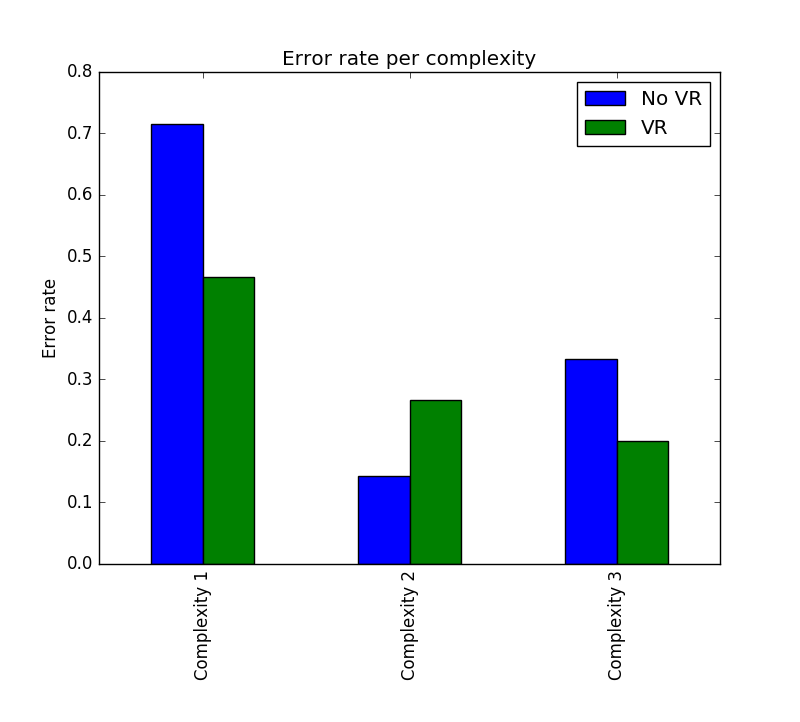
\includegraphics[scale=0.33]{image1.png}
\caption{Error rate per complexity level and condition} \label{fig:plot1}
\end{figure}

Figure \ref{fig:plot1} shows how the X axis is split up in three complexity
levels and the Y axis measures the average error rate in each complexity
level. The first interesting thing that can be observed in this plot is
that in the first and third complexity levels, the error rate produced
with no use of VR is higher than the error rate when the subjects used
VR to visualize the graph. This was expected because the use of VR
should make the task of visualizing graphs easier. However, in the
second complexity level the exact opposite happens. This result was
completely unexpected and it's difficult to make a conclusion about this
distortion.

If we take the mean percentage of correct answers, that is the
inverse of the error rate, the percentage that corresponds to the use of
VR is 68.89\%. This is slightly higher than the percentage of correct
answers without the use of VR, which is 60.47\%. This is not a big
difference in performance, but follows the tendency meassured in the
original paper.

On the other hand, independently of whether VR is used or not, the error rate in the
first complexity level is quite a lot higher than in the other two complexity
levels. This is the opposite of what we expected and what was found in
the original paper. That is, the error rate should increase
proportionally to the level of complexity. The explanation we can give for
this is that the subjects that perform the experiment for the first time
must get used to the device and the experiment, thereby taking longer in the first few attempts. This learning process takes some time that we didn't provide. Therefore, we could say
that this was an issue caused by the lack of familiarity with the device
and an issue in the design and execution of the experiment.

\begin{figure}[!ht]
\centering
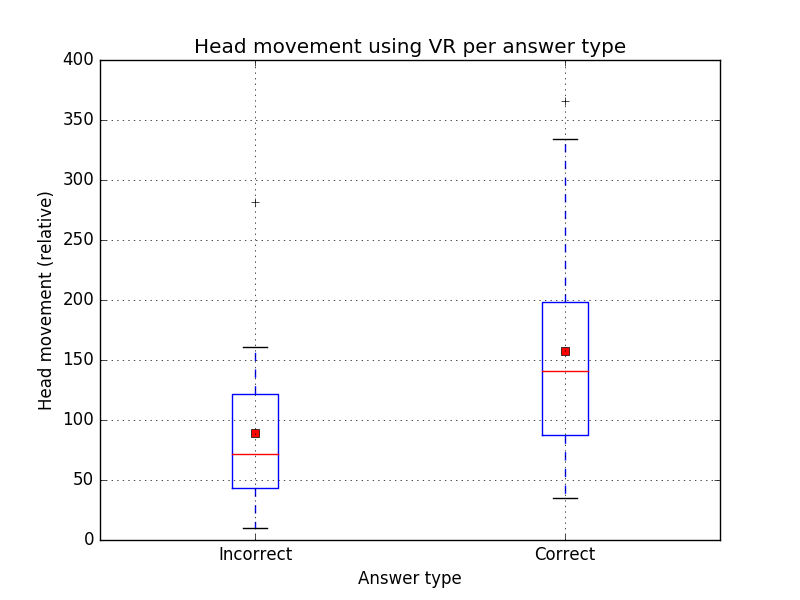
\includegraphics[scale=0.33]{image2.png}
\caption{Head movement using VR per answer type} \label{fig:plot2}
\end{figure}

In figure \ref{fig:plot2}, we can see the amount of head movement produced every time
a subject provided either an incorrect or a correct answer. This
relation wasn't discussed in the original paper and it provided some
interesting results. The main result was that the amount of head
movement increased by 30.19\% for correct answers with respect to
incorrect answers. That is, people that move their head more to
visualize the graph are more likely to give the correct answer. The head
movement was measured using the movement of the camera in the virtual
space in Unity units. It doesn't provide a reference to see the
real distance traversed by the head in meters, but it allows us to
compare among different scenarios and subjects.

\begin{figure}[!ht]
\centering
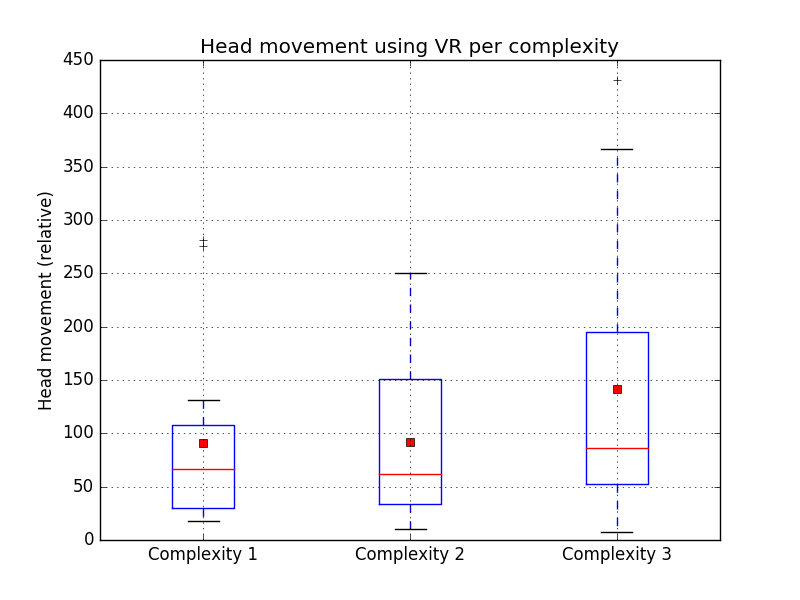
\includegraphics[scale=0.33]{image3.png}
\caption{Head movement using VR per complexity level} \label{fig:plot3}
\end{figure}

Similarly to the previous plot, in figure \ref{fig:plot3}  we can observe again the head movement in the
Y axis and the X axis is split up in three complexity levels. Specifically
for the third complexity level, the mean amount of head movement is
slightly higher than in the others. This was expected because the
experiment was set up such that subjects in higher complexity levels have
a higher maximum amount of time and thus, they tend to spend more time
and it results in a higher amount of head movement in total, on average (which follows from time, assuming a constant amount of movement per unit of time). It can be
seen as well that the variance is very high in the third complexity level
due presumably to the fact that people really liked the sensation of VR at
this point of the experiment and they moved their heads to take
advantage of the experience.

\begin{figure}[!ht]
\centering
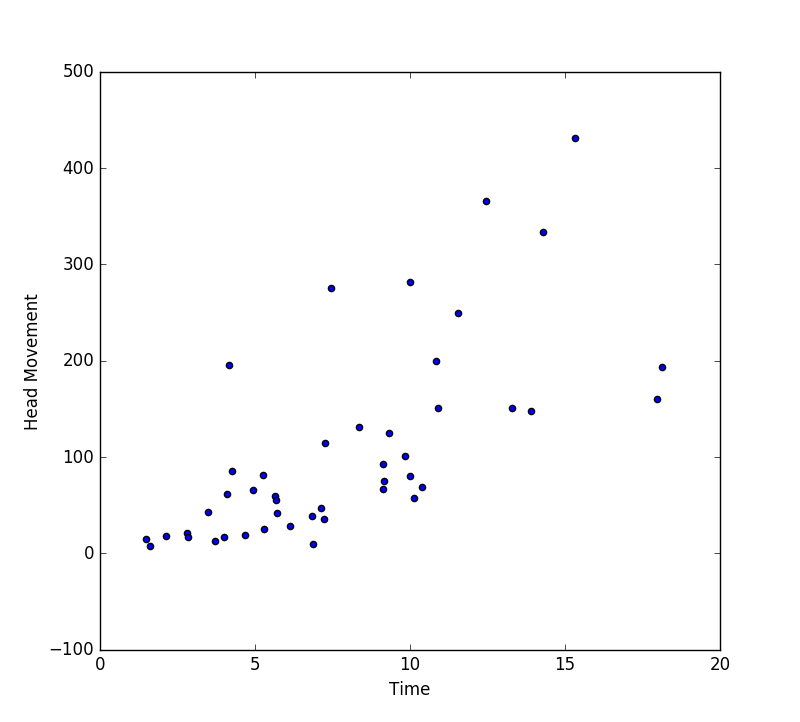
\includegraphics[scale=0.33]{image5.png}
\caption{Head movement and response time (in seconds)} \label{fig:plot5}
\end{figure}

In the scatter plot of figure \ref{fig:plot5} we can observe the same pattern of the previous
plot. Almost all the points are clustered in a range between 0 and 10
seconds and almost all of them have an upper bound of 100 units of head
movements. From this point, the variance starts to grow exponentially as
the time increases. This reaffirms the conclusion that when
people have more time to give an answer, they try to see the graph from
a different perspective to be sure that they are providing a correct
answer. Therefore. in scenarios where time is less of a constraint to
visualize the graph, people uses head tracking more to better comprehend
the graph.

\begin{figure}[!ht]
\centering
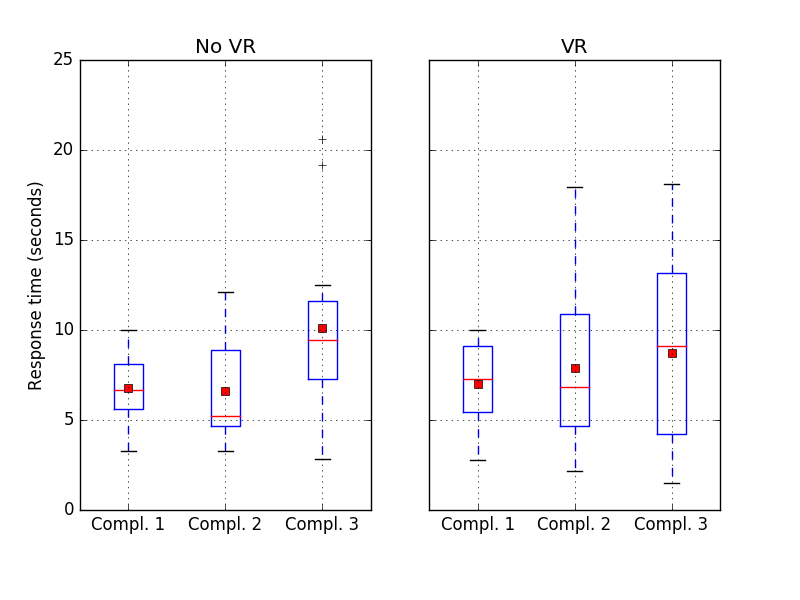
\includegraphics[scale=0.33]{image4.png}
\caption{Response time per complexity level} \label{fig:plot4}
\end{figure}

In the two box plots that are drawn in figure \ref{fig:plot4}, we can see the response time in seconds in the Y
axis, separated firstly in VR and no VR and secondly in the three
complexity levels. We can see for both plots that the higher the graph
complexity is, the higher the time a subject takes to answer. This
was of course expected because as the maximum time to answer increases,
people feel less pressure to make a decision. Therefore, we can't be
sure if the graph is really comprehended better or if it just
depends on the maximum amount of time provided to answer. This should
be compared with another version of the experiment in which the
information about the maximum amount of time is not provided and see the
real evolution.

We can also see that the variance in the response time is very high
again when VR is used. Again, we think that this is caused because
people really liked the VR experience and some of them spent longer on the experiment.
However if we observe the means and we compare them,
we can observe they are both practically the same in VR (7.81 seconds)
and No VR (7.88 seconds). Comparing to the paper, this is not what we
expected, which is that the response time should be lower when VR is used.

In all the plots we have analyzed, we can observer a common problem: The
sample size is too low to make significant conclusions. Several
technical problems and constraints in the availability of the device led
us to a partial failure in the data collecting. Some of the conclusions
we have made follow the tendency of the ones made in the provided
paper, but our results don't anywhere near the same level of significance as
those in the original paper.

For future work, if this experiment would be repeated, we would tweak
some of the parameters like the maximum amount of time to answer and the graph complexity increments, in addition to clearly informing the user about these values. Secondly, we would try to collect a much larger amount of data to get significant and reliable results that can really be compared to those in the original paper. Lastly, we would give our subjects some dry runs of the experiment, and time to get used to it. We would let them do more challenges per stage, and we would interview them about their experience afterwards.



